% 六、研究基础和工作条件。
% 保留已完成预实验与在研项目原始事实；未来工作量与methods.tex同步。
\subsection{与本项目相关的研究工作积累}
申请人颜丰为新疆大学副教授、博士、硕士研究生导师，已开展多模态视觉表征、特征交互及深度学习模型研究，可用于双时相表征、方法比较和训练评测。已有任务与矿山变化检测的标签及目标不同，迁移效果仍须专门验证。

在跨模态检索研究中，申请人作为通讯作者参与Feature Fusion Mamba Hashing via Decoupling方法的研究构思、方法设计、实验指导、结果分析及论文修改\cite{Tang2026Hashing}。表征分离和受控消融经验可用于分析变化与背景特征，矿山域泛化效果仍需检验。

在遥感视觉问答研究中，RSHR+工作涉及问题条件下的视觉校准和结构化状态空间推理，申请人作为通讯作者承担研究构思、方法设计、实验指导及写作\cite{Xu2026RSHR}，积累了遥感表征与实验经验。“视觉校准”属于任务相关的表征处理，不同于本课题的概率校准，预测可靠性需另行验证。

\subsection{已取得的研究工作成绩}
代表性成果还包括Knowledge-Aware Image Understanding with Multi-Level Visual Representation Enhancement，发表于\textit{Machine Learning}，申请人为第一作者及通讯作者，负责研究构思、方法设计、实验指导、分析与写作\cite{Yan2024Knowledge}。相关经验可用于本课题的问题定义、模型比较与结果解释。

\textbf{公开数据预实验（MCT-P01）。}2026年9月6日，基于MineNetCD作者发布的256像素裁切数据完成了三组对照\cite{Yu2024MineNetCD}。训练、验证四个分片均通过SHA256校验；按矿区及行号的固定哈希抽取50个训练矿区的1,188对影像和10个验证矿区的480对影像，矿区ID及完全重复影像对不交叉。采用118,593参数的轻量孪生网络，对无一致性约束、全区域约束、背景位置约束分别运行种子17、29、43；每组固定12轮、阈值0.5。同种子保持初始化、批次及增强一致，背景掩码只用于训练。九个末轮模型全部保存后统一评分，未按验证性能调参或选模型。

预实验执行流程见图\ref{fig:mct-pilot-workflow}。
\begin{center}
\begin{minipage}{\linewidth}
  \centering
  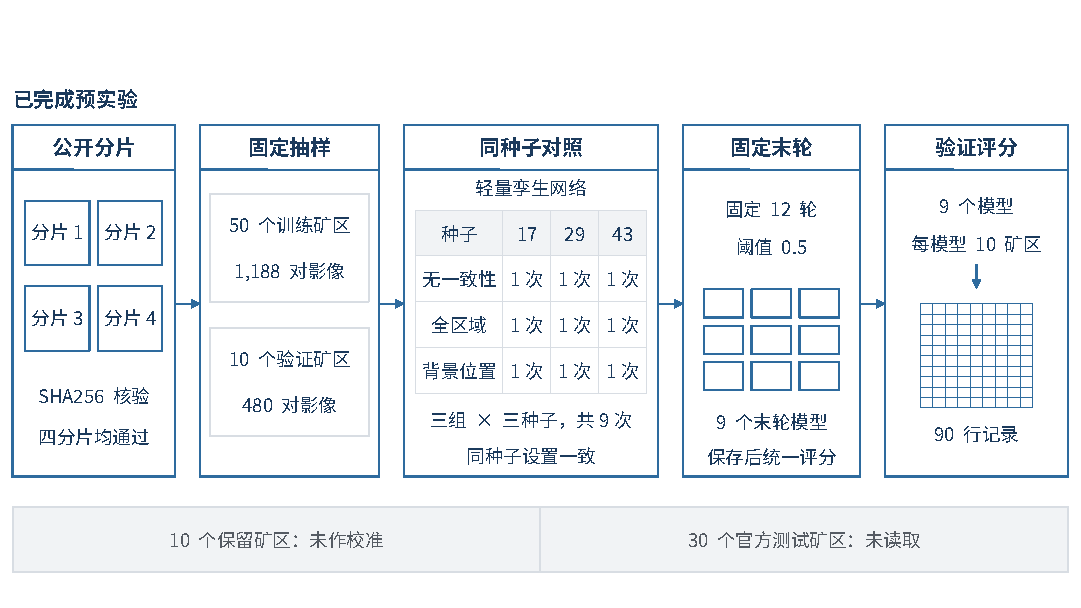
\includegraphics[width=\linewidth,trim=0 0 0 12mm,clip]{figures/vector/F14_pilot_workflow.pdf}
  \captionsetup{justification=justified,singlelinecheck=false}
  \captionof{figure}{已完成预实验流程。固定抽取1,188对训练影像和480对验证影像，运行三组各三个种子后统一评分。九个模型在10个验证矿区形成90行记录，真实结果见图\ref{fig:mct-pilot-results}。10个保留矿区未作校准，30个官方测试矿区未读取。}
  \label{fig:mct-pilot-workflow}
\end{minipage}
\end{center}

每矿区先汇总像素计数，再等权平均；下表为三个种子的均值，单位为百分数。完整种子离散程度、90行矿区计数和权重哈希已归档，三组比较与矿区配对效应见图\ref{fig:mct-pilot-results}。
\begin{center}
\begin{tabular}{lrrr}
\hline
训练约束 & 变化IoU & 背景误报率 & 总体召回率 \\
\hline
无一致性约束 & 21.08 & 24.13 & 67.82 \\
全区域约束 & 20.96 & 26.62 & 72.65 \\
背景位置约束 & 21.72 & 23.28 & 68.55 \\
\hline
\end{tabular}
\end{center}

按矿区内先平均种子、再配对bootstrap 10,000次计算探索性95\%区间。背景相对全区域的IoU差为$+0.76$个百分点，区间$[-0.06,1.52]$跨零；背景误报率差为$-3.35$个百分点，区间$[-4.22,-2.57]$，同时总体召回差为$-4.11$个百分点，区间$[-6.24,-2.23]$。降误报伴随召回下降；相对无约束的IoU和误报率差区间也跨零。预先定义的片内、不接边且面积不超过64像素的8连通变化区在验证子样本中为零，小变化召回不可估计，未事后改变阈值。

\begin{center}
\begin{minipage}{\linewidth}
  \centering
  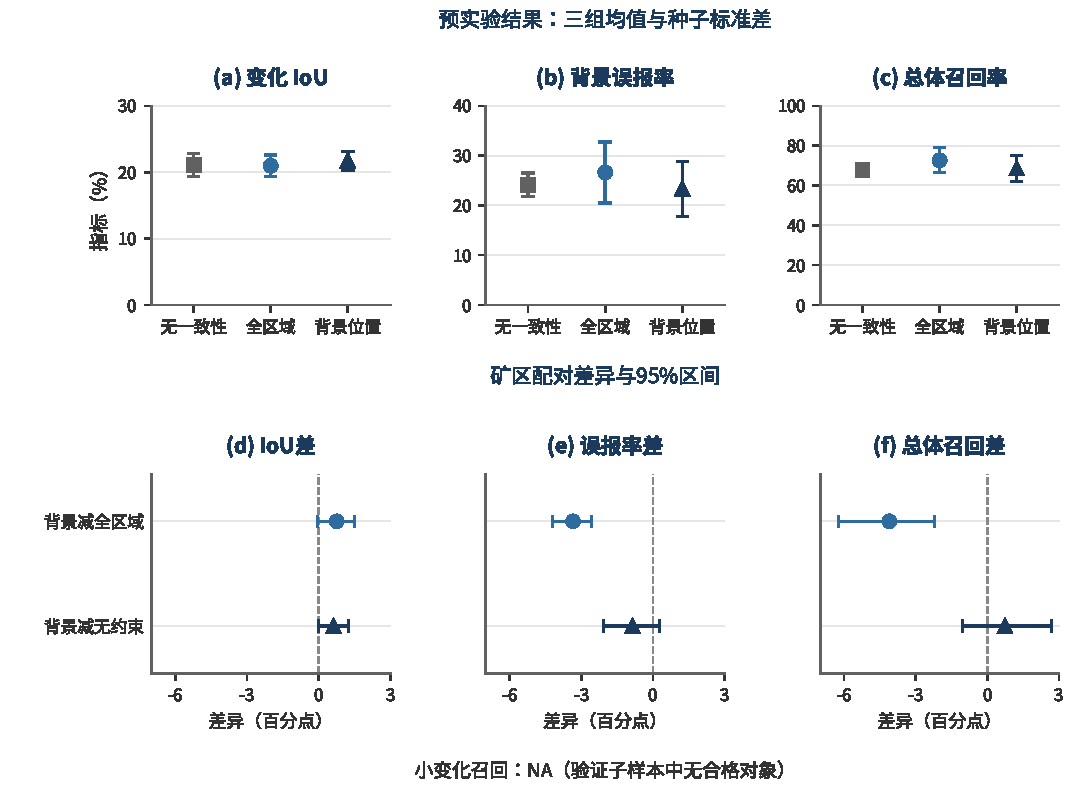
\includegraphics[width=\linewidth]{figures/F15_F16_pilot_results.pdf}
  \captionsetup{justification=justified,singlelinecheck=false}
  \captionof{figure}{预实验结果与矿区配对效应。上排为三个种子的矿区宏平均及种子样本标准差，单位为\%；下排先在矿区内平均种子，再对10个矿区配对重采样，展示差值及95\%区间，单位为百分点。背景相对全区域的降误报伴随总体召回下降；相对无约束的三项区间均跨零，小变化召回为NA。}
  \label{fig:mct-pilot-results}
\end{minipage}
\end{center}

该预实验提供了可复现的矿山数据运行及误差证据，但尚不支持“降误报并保持细小变化检出”的联合假说。当前仅约束背景位置，深层特征仍可能感受邻近变化区；相同权重也不保证实际梯度强度相同。后续需核验原始场景的小变化端点，完成DonaNet、随机掩码和强度匹配对照。完整版归档、官方测试和可靠性实验尚未完成。

\textbf{外观差异代理量的可计算性与混杂（MCT-P01-EXT-Ds）。}在同一批480个验证切片上计算了本申请所定义的外观差异代理量$D_s$，归一化与腐蚀口径与上述预实验一致，逐样本哈希全部校验通过；该扩展不训练模型，误差数值取自上表所依据的逐矿区结果，官方测试矿区同样未读取。474对可计算$D_s$，6对因腐蚀后无有效未变化像素记为不适用，矿区级$D_s$跨度0.0915—0.2196。按矿区$D_s$中位数分档，三组约束下高档的背景误报率均高于低档（背景组低档19.07\%、高档27.49\%），方向符合预期，但$D_s$与背景误报率的Spearman相关置换检验p值在0.28—0.57之间，10个矿区不足以支持确认性结论。

需要在正式方案中处理的是一处混杂：高$D_s$档的变化IoU同样更高（背景组低档17.83\%、高档25.61\%），与“外观差异使任务更难”的朴素预期相反。检查发现$D_s$与矿区变化像素占比同向共变（Spearman $+0.370$，置换p=0.295），低档矿区平均变化像素占比7.24\%、高档13.06\%。变化像素占比直接影响IoU的分母结构，因此按$D_s$分层的组间差异不能单独归因于外观差异。正式实验按$D_s$分层时将同时报告各档的变化像素占比，分层结论以背景误报率为主，不用变化IoU解释外观差异的作用。

\subsection{研究风险与应对措施}
\textbf{数据与语义风险。}若归档无法追溯矿区和原始场景，暂停未见矿区泛化结论，核实来源或改用可溯源的分组实验。配准和标签争议主导误差时，记录质量问题与敏感性结果，收窄解释范围；剔除规则不得依赖测试性能。

\textbf{机制与效果风险。}若背景约束损伤小变化召回，或优势仅来自强度、阈值变化，不将其作为区域选择有效的证据，保留权衡及反例。正式小变化端点不足20个有效测试矿区或100个完整分量时仅作描述，不扩大面积界点。相对全图改善而未优于无约束时，只报告两种约束的相对差异；排序无增量时分析残留错误，不叠加复杂模块。负结果仍按预定对照形成条件性结论。

\textbf{实施与产出风险。}共享算力、人员投入和审稿周期可能影响进度。按实测耗时排期，优先主比较和强度对照，再完成DonaNet适用性比较，必要时缩减外部扩展。写作与实验同步，预留修改及发表时间；中期和结题节点按实验室安排执行，投稿不能代替源刊论文发表。

% 以下迁自原稿 3.2.工作条件.tex。
\subsection{已具备的实验条件}
申请人确认可稳定使用NVIDIA A40显卡8张和NVIDIA GeForce RTX 3090 Ti显卡6张，具备Linux、Python、深度学习框架、Git及LaTeX工具链，可支持公开影像处理、单卡与多卡训练及多种子评测，但非本课题独占。MCT-P01已在单张A40完成九组训练，纯训练合计约558秒，不含数据准备与验证；正式实验仍须按模型规模和可用时段计时、排期。

已取得作者公开的MineNetCD256训练与验证四分片并核验SHA256，保存固定抽样清单、代码、模型和逐矿区指标供复查MCT-P01。完整版MineNetCD归档未完整验收，官方测试影像未读取；EuroMineNet及全球铜矿数据仅完成来源与许可核查。正式实验需追溯原始场景、切片位置及配准质量，按许可登记引用与衍生产物公开范围。

% 以下迁自原稿 3.3.承担项目情况.tex。
\subsection{正在承担的相关科研项目及与本课题的关系}
\label{sec:mct-ongoing-projects}

本申请借鉴以下项目的建模与数据整理经验，聚焦矿山双时相变化检测与复核评价，拟单列数据来源、实验记录及论文结果。

\textbf{（1）融合多源数据大模型驱动的光伏发电功率预测方法研究。}自治区高校基本科研业务费科研项目培育类，批准号XJEDU2026P005，经费5万元，执行期2026年1月至12月，申请人主持，负责总体方案、模型研究和成果组织。其任务为光伏功率预测；本申请拟另设矿山变化定位的数据划分与误差指标。

\textbf{（2）多模态融合技术研究及其在新疆产业集群中的应用。}自治区天池英才引进计划青年博士人才项目，经费50万元，执行期2025年2月至2028年2月，申请人主持。本申请围绕矿山双时相影像开展区域约束、独立矿区校准与固定面积复核评价。

\textbf{（3）面向政企数字化应用的智能知识库与问答系统研发。}新疆数字云创有限公司委托的横向课题，编号202604140013，经费12万元，执行期2026年6月至10月，申请人主持，按合同构建知识库，成果及知识产权由合同双方共同享有。本申请拟另行形成矿山变化检测与复核代码；合同代码如需使用，按原授权及共享约定执行。

\textbf{（4）数据驱动下基于互补型生成对抗网络与神经统计模型的公路沙害智能预警研究。}国家自然科学基金地区项目，批准号62466056，经费32万元，执行期2025年1月至2028年12月，申请人作为参与者负责数据收集整理，基金委登记单位为新疆大学。数据整理经验可用于矿区与切片溯源；本申请拟单列MineNetCD清单、标签核验和误差统计。

\textbf{（5）可学习乘积量化与状态空间模型协同的长上下文高效注意力机制研究。}中国人工智能学会（CAAI）—蚂蚁科研基金，编号202604140006，经费15万元，执行期2026年2月至2027年2月，申请人参与，负责高效注意力机制研究。本申请借鉴高效建模经验，沿用轻量骨干，重点评价约束区域与错误排序对检测、复核结果的影响。
